\chapter{Evaluation}\label{ch:evaluation}
For our tool, usability and user experience are very important. Therefore, we did two user studies. The first was to test the usability of GuideaMaps 2.0 (as map creator and as end-user), while the second study more specifically evaluated whether the visualization provided for Plateforme DD was an improvement over the original structure provided on the website.\\

This chapter is divided in two sections. The first describes the user study of GuideaMaps 2.0 together with its results. In the second section, the same is done for the user study of Plateforme DD.





\section{GuideaMaps}
In this section, we describe the evaluation of the default implementation of the tool. With ``default'' we mean that no implementation is plugged into the library but the standard visualization is used as described in \autoref{sec:default-implementation}.

\subsection{Setup}
The evaluation was split in two parts, each evaluating one of the two modes. In the first part, we evaluated the map creator mode with eight participants. Because GuideaMaps is intended for the requirements elicitation of domain-specific software, the map creators will in general be people from the domain of Computer Science. Therefore, we asked people with a background in Computer Science and/or visualization techniques to participate. However, the users that will provide the actual requirements can be almost everyone. Therefore, a Computer Science background was not a requirement to participate in the part evaluating the end-user mode, which was evaluated by eight participants. All participants for the evaluation of both modes were unique, i.e. there was no participant who evaluated both modes.\\

All participants answered the questions at home without additional explanation than the text provided at the beginning of the questionnaire.

\subsection{Tasks \& Questions}
For the two modes, a different (online) questionnaire was created (see \autoref{appendix:gm-evaluation-map-creator} and \autoref{appendix:gm-evaluation-end-user}). Both questionnaires start with a brief explanation about the tool.\\

Next, the participant was asked for his age and whether he had a background in Computer Science and/or visualization techniques or not. These general questions were followed by a number of tasks the participants had to perform followed by some questions.\\

The goal was to let the participants experience the actions a real map creator or end-user can perform. After each action, we asked to indicate how intuitive it was for them to obtain the requested result. We asked this question because we want the tool to be usable without much explanation or training. When the majority of the participants would indicate that a certain action was not intuitive at all, we know something should be changed in the design of the tool. After all these tasks were finished, the participant was asked to upload a screenshot of his screen, so that we can check whether everything went as intended.\\

Furthermore, to obtain a general idea of the usability of the tool, the participants were afterwards asked to fill out the SUS usability questionnaire\footnote{\url{https://www.usability.gov/how-to-and-tools/methods/system-usability-scale.html}}. We chose for this questionnaire because, according to a study of \cite{tullis2004comparison}, SUS gives the most reliable results in comparison to other questionnaires (e.g. QUIS and CSUQ). Further, SUS is the only questionnaire of the ones they studied that addresses multiple aspects of the user's reaction to the system (in their case a website), while other questionnaires ask more about specific features of the system.\\

The questionnaire was concluded with some open questions. We asked to tell us what was good about the visualization and where they think we could have done better.

\subsection{Results}
Because there are different questionnaires for the two modes, the results are separated in the next two sections. For the questions about the intuitiveness of the task, we only discuss remarkable results or questions of which the result was (absolutely) not intuitive.

\subsubsection{Map Creator}
The first task to evaluate the functionality of the map creator was to provide a title to the root node. We see that 25\% of the participants indicated this action was not intuitive and another 25\% were neutral about the intuitiveness of this task. A frequently returning remark was that participants tried to click on the title to edit it. They also said they did not link the magnification icon to editing possibilities. Suggestions for better icons were a gear or a pencil. Hence, we should consider to replace the magnifier icon with a better icon.\\

The other tasks were evaluated as intuitive to very intuitive, with some exceptions indicating \textit{neutral}. However, the task to delete an option of a choice node was not intuitive for 87,5\% and absolutely not intuitive for 12,5\% of the participants. This means we could have done much better for this functionality. A comment we encountered frequently was that a small button to delete an option would be much more intuitive than having to delete the title and description. Now, the functionality is somewhat hidden and difficult to find. Another remark about buttons is that the position of the button to delete a node was weird.\\

Finally, the participants answered the ten SUS questions and the results are satisfying: the average score is 72,5 on 100. 

\subsubsection{End User}
As already mentioned, different tasks and questions were prepared to evaluate the functionality provided to the end-user. In the first task, it was asked to add content to a specific node. While 75\% experienced this as a (very) intuitive action, 25\% found it not intuitive. This has possibly a similar reason than in case of the map creator: the participants probably clicked on the place of the node where the content should be visible, but could not insert the content from there.\\

Further, when some options of a choice node are selected, child nodes are added to the visualization. We asked the participants to delete one of these options. While 5\% indicated this action is (very) intuitive, 25\% experienced the same action as not intuitive and 25\% as neutral. Hence, deleting an option was not super clear for half of the participants.\\

We also asked whether the participants understood the meaning of the ``completeness-icon'' (without calling it like this to not reveal the answer). Some of the answers were quite close to the correct interpretation but no participant could give a completely correct explanation. The same situation took place for the question about the lock symbol. To solve this issue, some participants suggested to provide a document with guidelines explaining possible actions and the meaning of elements like the completeness-icon.\\

In the end, the participants answered the ten SUS questions and with an average score of 69,375 on 100, the result is slightly lower than the one of the map creator.

\subsubsection{Overall}
In general, the user studies yielded important information. First of all, we have to be even more careful than we expected with the icons we use for actions (\ref{ur:icons}). We saw that users do not click on a button if they are convinced it is not meant for what they are searching for. Even though some participants mentioned the tooltips were helpful, some of them probably did not notice them and misunderstood the meaning of the icons.\\

In the future, deleting elements should always be done via a button. Other ways are not intuitive (enough). Further, a frequent remark was that participants tried to click on the title or the content of a node to change it. Hence, it would be useful to be able to change it in this way instead of having to open the modal for every change.\\

As a conclusion, we can say that our application scores reasonably well in terms of usability. However, some issues need to be solved to improve the tool (e.g. icons, guidelines).




\section{Plateforme DD}
The goal of the evaluation of the Plateforme DD use case (\autoref{ch:usecase}) was different in comparison to the one about GuideaMaps. Here the goal was to investigate whether our visualization would be easier to use and understand than the current website\footnote{\url{https://sciences.brussels/dd/}} of Plateforme DD for the target audience, being pupils from secondary schools.\\

In this evaluation, the participants were around 15 years old. This age group was chosen because the content on the current website was created by youngsters of similar ages. Note that the participants of this user study never worked with the website before.

\subsection{Setup}
We divided the participants into an experimental and a control group. The control group solved the questionnaire using the website, while the experimental group solved the same questionnaire using our application.\\

There was one tablet per two children on which the website or the application was running (depending on the group they were in). Note that they did not work with both systems to avoid a learning effect (having used one system could influence the results for the other system). 

\subsection{Tasks \& Questions}
The user study consisted of different questions the children had to answer for which they had to explore or search in the system. Before they started with the actual tasks, we gave them five minutes to explore the system, i.e. the website or the application, so that they could become somewhat familiar with the system. We mentioned that it was important to understand the structure as much as possible because some questions would follow after this introduction period.\\

After five to ten minutes, we distributed the papers with the tasks and the questions. With other words, all children (of both groups) received part 1 of the questionnaire (see \autoref{appendix:pdd-questionnaire}). The first six questions of part 1 intended to test the understanding of the structure of the content. Then, four more questions were added to test the ease of searching and finding information in the system. The participants using our application also had to answer four more questions to measure their understanding of the visualization approach used.\\

After twenty minutes, all questionnaires of part 1 were collected, even if the participant did not finish all questions yet. Together with the questionnaires, the tablets were collected, as they were not needed anymore for part 2 of the user study. After collecting everything, part two of the questionnaire was distributed to all participants. In this part, the questions were not about the content or the structure of the information, but about usability and user experience. We did this because we also wanted to be able to compare the results about usability and user experience of the two systems. The questions about usability and user experience can be found in \autoref{appendix:pdd-questionnaire} and \autoref{appendix:ueq-questionnaire}, respectively. The usability questions are based on the SUS questionnaire previously mentioned, but adapted a bit because not all questions were relevant for our purpose. To evaluate the user experience, we used the UEQ questionnaire\footnote{\url{https://www.ueq-online.org/}}.



\subsection{Results}
In general, we hypothesize that participants using our application answer more of part 1 correctly than the participants using the website.\\

Note that the participants only got 20 minutes to answer all questions. We expected that not all participants using the website would be able to answer all questions in this amount of time. Even though we know it is possible that some participants using our application would also not be able to finish the questionnaire either, we predict that participants using the application will be able to answer more of the questions than participants using the website.

\subsubsection{Structure Comprehension}\label{sec:evaluation-pdd-structure-comprehension}

\begin{figure}[H]
	\centering
	\frame{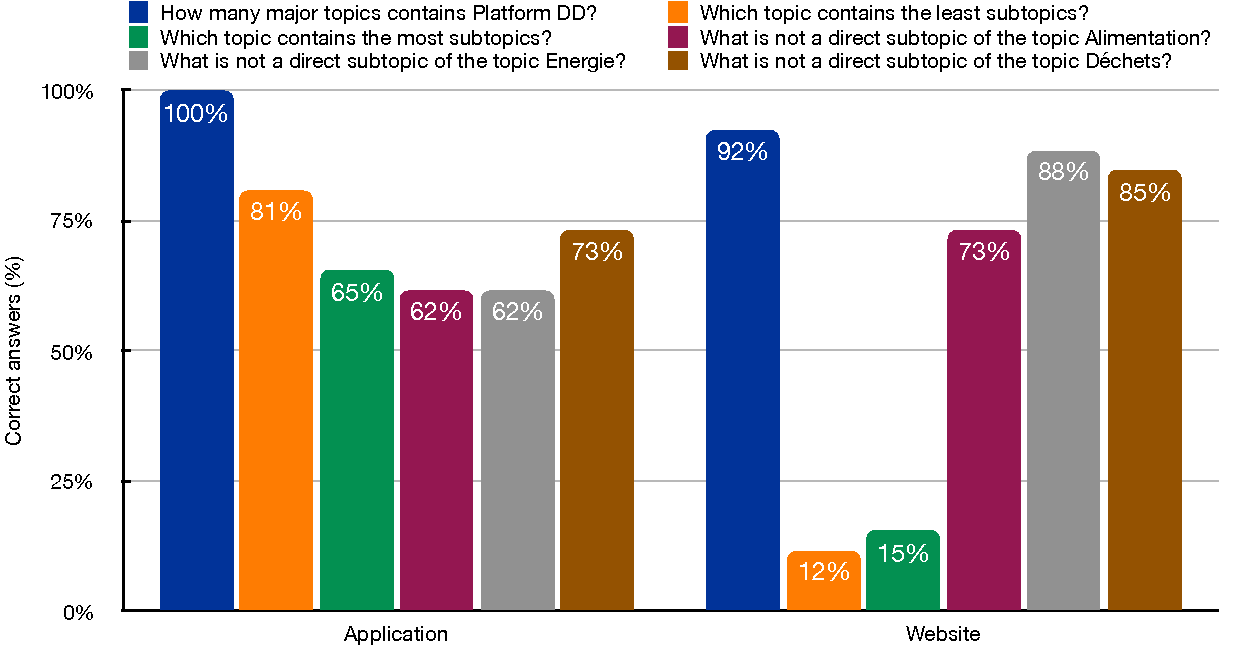
\includegraphics[width=\linewidth]{evaluation/part1-first6.pdf}}
	\caption{Results of the first 6 questions of part 1.}
	\label{fig:evaluation-pdd-first6}
\end{figure}

\autoref{fig:evaluation-pdd-first6} shows the results of the first six questions of the questionnaire. We can see that almost every participant correctly found that the content is divided over three major topics.\\

Participants using our application were significantly better in finding which topic contains the most and which the least number of subtopics. We expected this because in our application, the tree structure is more clear. As a consequence, these users have a better overview than the participants using the website.\\

To the questions about which topic is not a direct subtopic of a certain topic, the participants using the website gave a correct answer more frequently. This is probably because these users cannot see the indirect subtopics of the topics in the questions. Participants using our application possibly made some indirect subtopics visible by clicking on the plus-button.

\subsubsection{Search \& Find}
The results to search and find related questions can be found in \autoref{fig:evaluation-pdd-search-find}. In general, we see that participants using our application are better in retrieving the information than the ones using the website. However, in one question participants using the website were slightly better in finding the correct result, but the difference is almost negligible.

\begin{figure}[H]
	\centering
	\frame{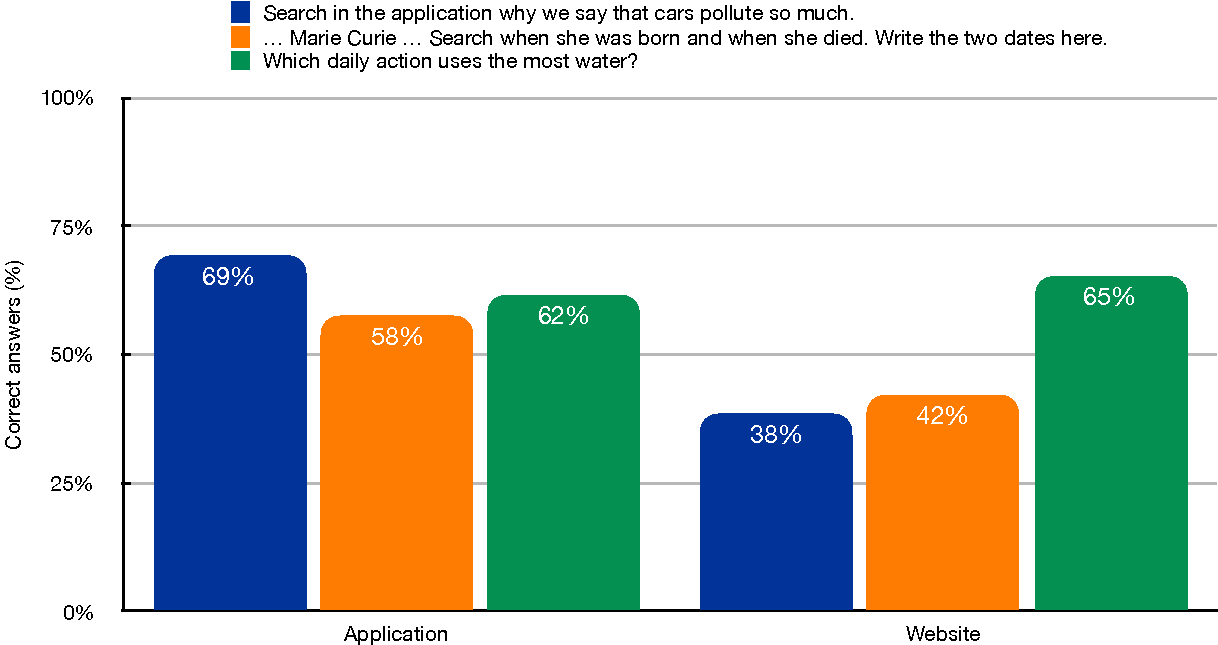
\includegraphics[width=\linewidth]{evaluation/part1-search-find.pdf}}
	\caption{Results of search \& find questions.}
	\label{fig:evaluation-pdd-search-find}
\end{figure}

We also asked them to write as much titles as possible of topics that are still ``under construction''. This was not very successful because more than half of the participants could not find such a topic. The average number of topics found per participant is 0.42 in the case of our application and 0.81 in case of the website. This is probably because going through the topics on the website is quite fast, i.e. you just click on other topics until you find one that is under construction, while in our application you have to open and close the nodes one by one which takes more time.\\

In general, when looking at \autoref{fig:evaluation-pdd-first6} and \autoref{fig:evaluation-pdd-search-find}, we can conclude that our hypothesis was correct, i.e. participants using our application answer more questions correctly. Furthermore, in case our application has more correct answers, it outperforms the website almost every time. Hence, our application certainly is better than the website for structure comprehension (\autoref{sec:evaluation-pdd-structure-comprehension}) and searching and finding information.

\subsubsection{Understanding of the Visualization}
The participants using the application had to answer four additional (multiple choice) questions to test their understanding of the visualization. The results (\autoref{fig:evaluation-pdd-insight}) make clear that most of the participants understand that subtopics give more detailed information about their parent node when a concrete example is used. However, when this question was formulated in a more general way (question B), a lot of the participants were wrong or indicated they did not know the answer. Even though the answer was almost revealed in question D (\textit{A click on the plus-button of a bubble allows me to find projects on more specialized topics for that bubble}), only 35\% found the correct answer.\\

Many participants did not know the answer on question C, which was about the cross references (\textit{There is no connection (arrow) between the bubble ``Les d\'echets dans la nature'' and the bubble ``La pollution atmosph\'erique''. However, are these topics in some other way related?}). Only 38\% of the answers on this question was correct.\\

Hence, we were not very successful in testing the understanding of the visualization. There are two possible explanations. Either, the youngsters did not understand the visualization or the level of abstraction used in those questions was too high for them.

\begin{figure}[H]
	\centering
	\frame{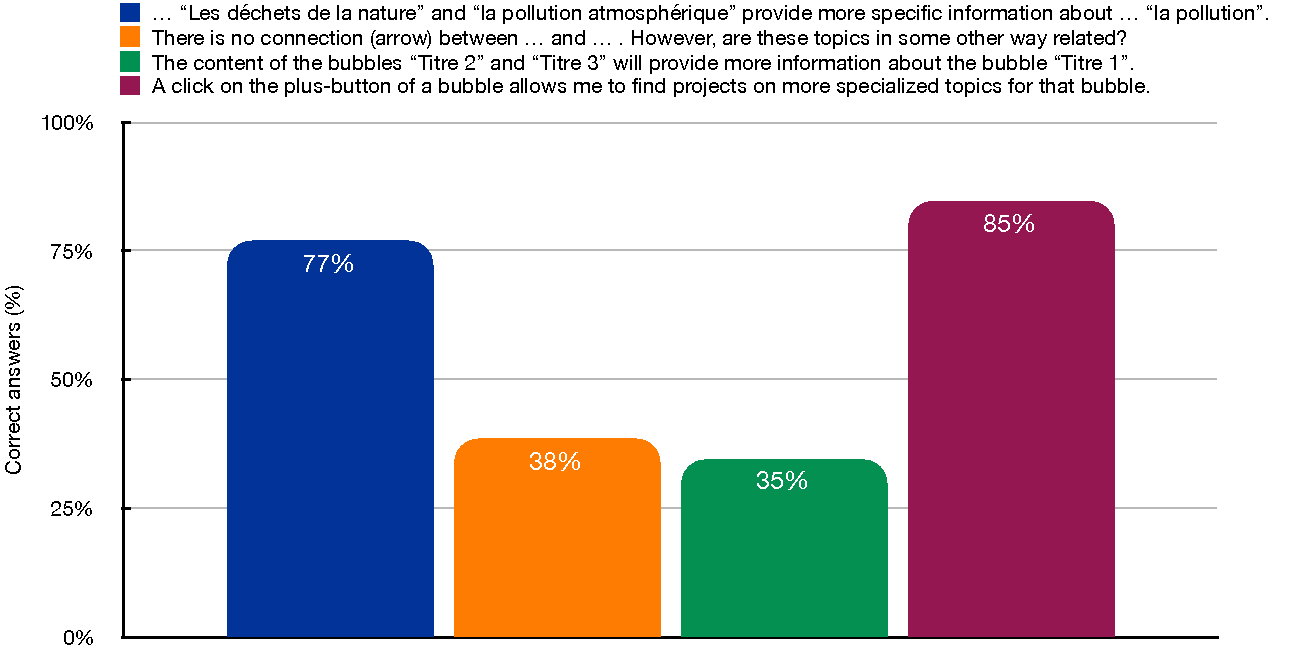
\includegraphics[width=\linewidth]{evaluation/part1-insight.pdf}}
	\caption{Results of questions about understanding of the visualization.}
	\label{fig:evaluation-pdd-insight}
\end{figure}




%\begin{figure}[H]
%	\centering
%	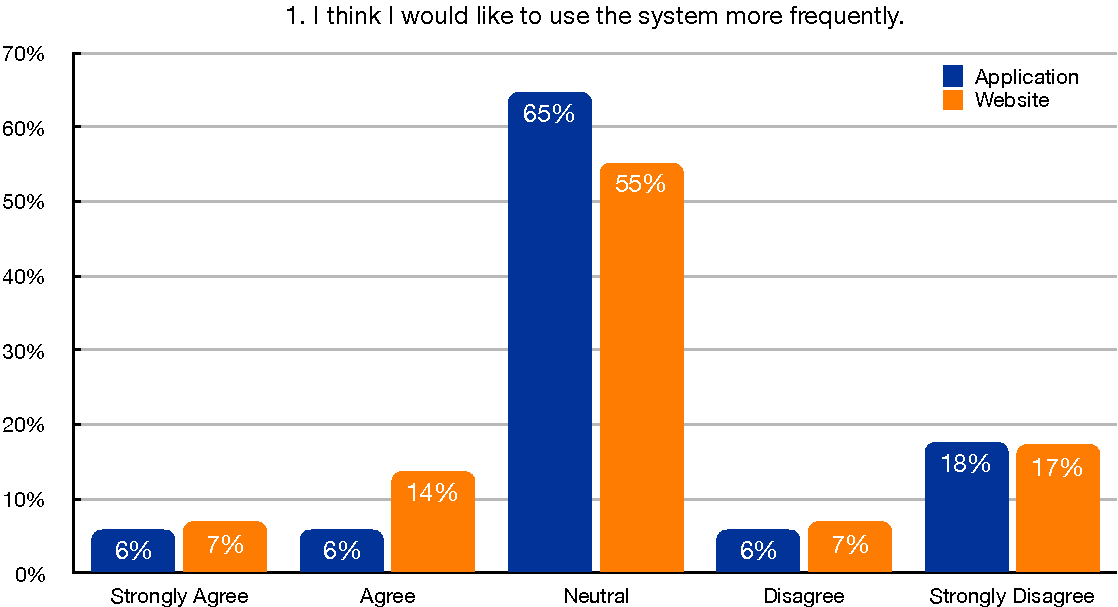
\includegraphics[width=.49\textwidth]{evaluation/usability-q1.pdf}
%	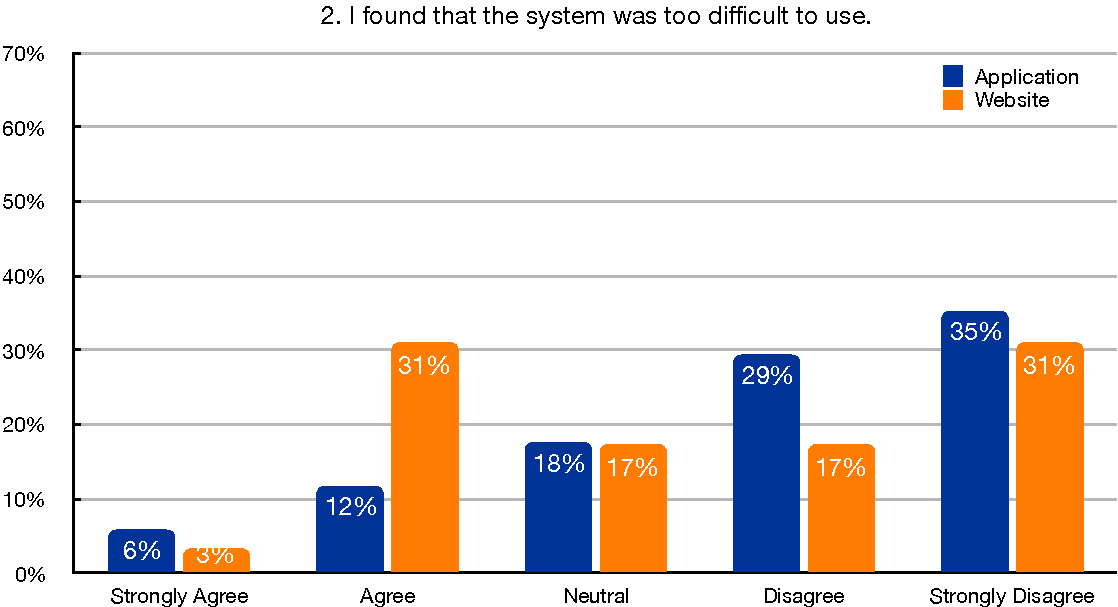
\includegraphics[width=.49\textwidth]{evaluation/usability-q2.pdf}
%	
%	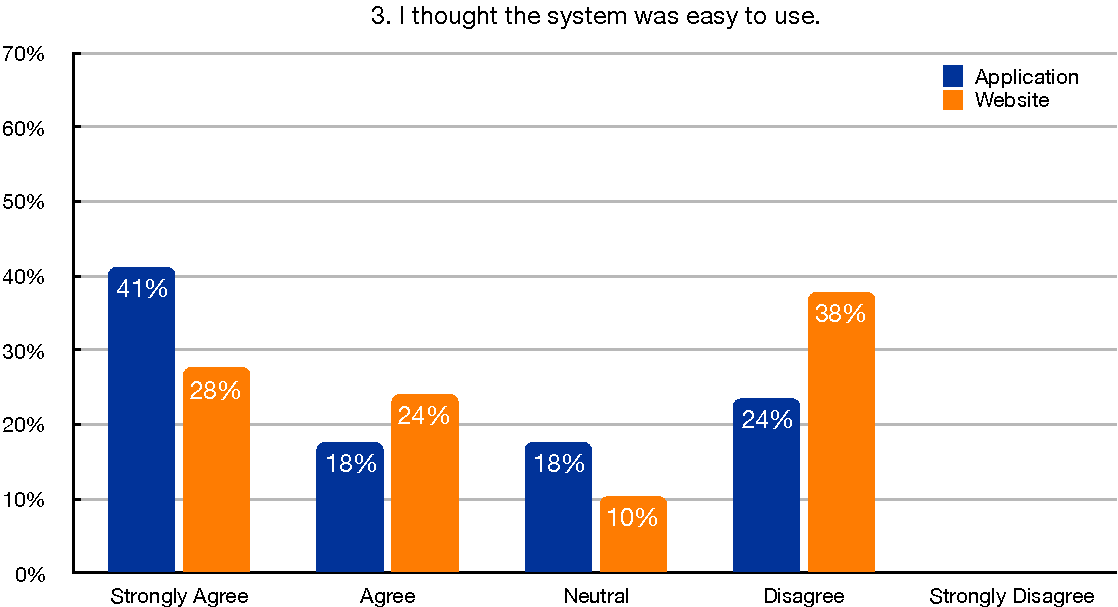
\includegraphics[width=.49\textwidth]{evaluation/usability-q3.pdf}
%	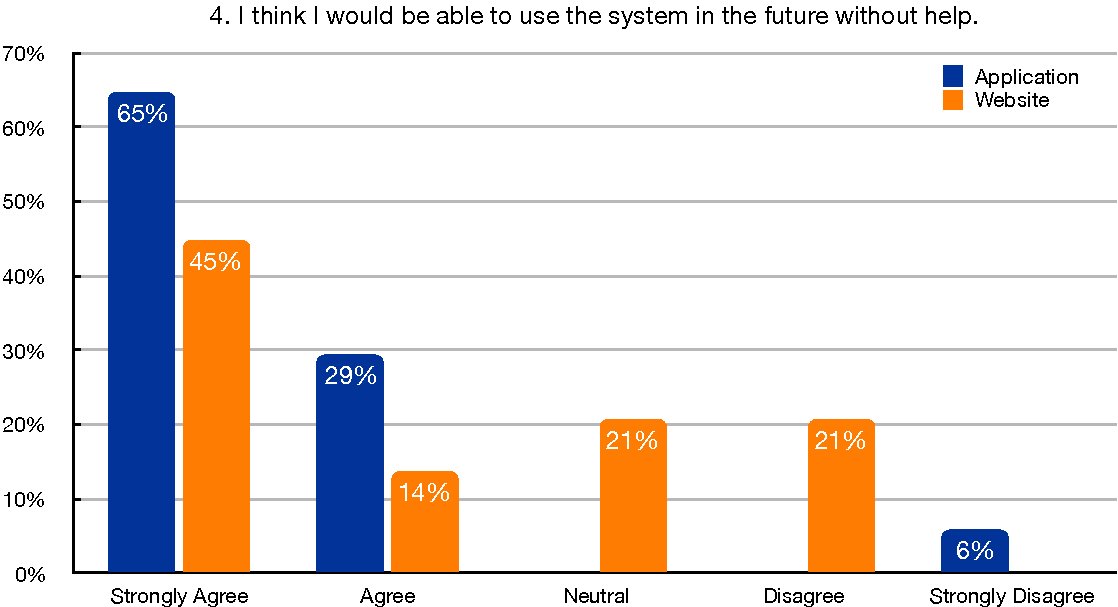
\includegraphics[width=.49\textwidth]{evaluation/usability-q4.pdf}
%	
%	\caption{test}
%\end{figure}

\subsubsection{Usability}
For the second part, we hypothesize that the website is less usable than our visualization and that our application provides a better user experience.\\

\autoref{fig:evaluation-pdd-usability} shows eight graphs, each representing the results of one of the eight questions about usability of Plateforme DD. When we look at the results of the first question, we can conclude that most of the participants (in both groups) are not very sure about whether they want to use the system more frequently or not.\\

In question two and three, we asked about the simplicity of the website or our application. We see that the majority of the participants using our application (strongly) disagrees with the statement that the tool is too difficult to use. On the other hand, we see a peak of participants using the website who agree with the same statement. In the next statement, the opposite was asked. Here we can make similar conclusions. In case of our application, the majority answered this question with ``strongly agree'', while in case of the website an equal percentage answered ``disagree''. Hence, based on these two questions, we can conclude that our application was easier to use than the website.\\

Furthermore, almost all participants using our application (all except 6\%) think they will be able to use the tool in the future without help. In case of the website, 42\% is neutral or disagrees with this statement. The fifth question enforces this result even more: 82\% of the respondents using our application thinks their friends would be able to learn the system quickly, while in case of the website this is only 49\%.\\

We see that participants using our application agree quite often with the sixth question, ``I found it too much hassle to use the system'', while the majority using the website disagrees with this statement. This is probably because our application was slower than expected on the used tablets. As a consequence, the tool was not always responding immediately, which was sometimes confusing for the users.\\

From the results of the seventh question, we can see that participants using the website were a bit more self-assured than participants using our application. In the last question, the distribution of the answers was similar for both systems, i.e. the majority did not need a lot of time before they could use the system smoothly.\\

Overall, based on the answers from this usability questionnaire, we can conclude that our application scores slightly better on usability than the website. Hence, by creating the tool we succeeded in our intention to make the structure of the content more clear and more attractable than the website. This is supported by a note on the form of a participant using the website: ``I don't understand it''.



\subsubsection{User Experience}
To evaluate the user experience, we used the UEQ questionnaire\footnote{\url{https://www.ueq-online.org/}} (\autoref{appendix:ueq-questionnaire}) composed in such a way that inconsistencies can be easily detected. Together with the questionnaire, an excel-file is available that allows to analyze the answers and to create graphs.\\

The questionnaire consists of 26 terms at one side with their opposite at the other side, e.g. annoying versus enjoyable. A number between one and seven is used to give a score to this criterion. Each couple of terms, i.e. criterion, corresponds to one of six categories: attractiveness, perspicuity, efficiency, dependability, stimulation, and novelty.\\

The excel-file converts the numbers from one to seven to a range between -3 and +3, where -3 stands for the most negative answer and +3 for the most positive answer of the two. For each couple of opposites, the mean is calculated based on the converted answers, resulting in a number between -3 and +3. Because it is very unlikely to have a mean lower than -2 and higher than 2, the graphs are given with a range between -2 and +2. The resulting graphs can be found in \autoref{fig:evaluation-pdd-ueq}.\\

\begin{figure}[H]
	\centering
	\begin{subfigure}{.49\textwidth}
  		\centering
  		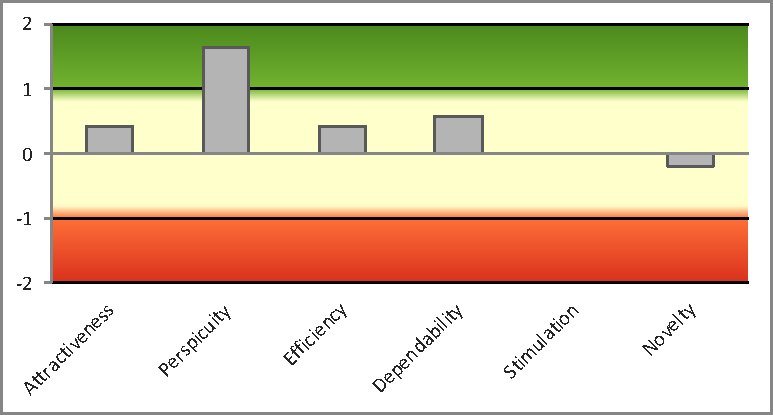
\includegraphics[width=\linewidth]{evaluation/evaluation-pdd-ueq-app.pdf}
  		\caption{Results User Experience Application}
  		%\label{fig:plusicon}
	\end{subfigure}%
	\begin{subfigure}{.49\textwidth}
  		\centering
  		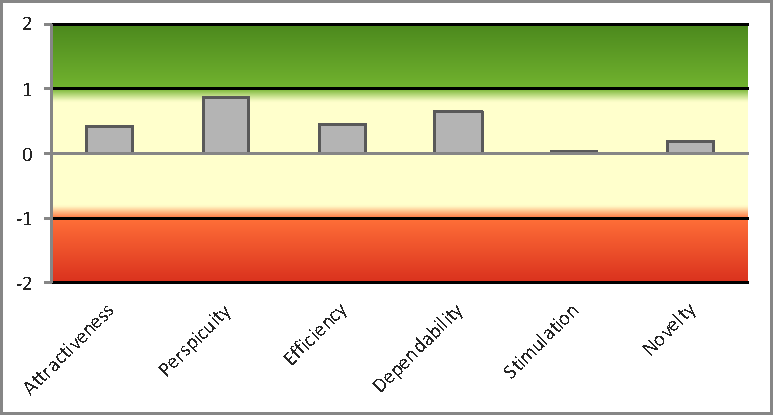
\includegraphics[width=\linewidth]{evaluation/evaluation-pdd-ueq-website.pdf}
  		\caption{Results User Experience Website}
  		%\label{fig:editicon}
	\end{subfigure}
	\caption{User Experience Results Plateforme DD.}
	\label{fig:evaluation-pdd-ueq}
\end{figure}

We can see that the score for the perspicuity of our application is higher than the one for the website, which means the application is more clear. A remarkable result is the one for efficiency: the application seems to be less efficient than the website. Maybe this can be explained as follows. The majority of the respondents indicated that our application was slow. As already mentioned, this is due to the devices used, but it was very inconvenient for them and this probably influenced the score for efficiency.\\

Further, we also see that our application scores significantly lower for novelty than the website. We think this is mainly due to the answers on the ``dull/creative''-criterion. Participants using the website found the website more creative than the respondents using our application, which has its impact on the score for novelty.\\

The score for stimulation is average because the criteria concerning stimulation most of the time got scores between three and five. The score for dependability is a bit higher in case of the website. This is probably because our application was quite slow on the tablets, which had as a consequence that it not always met expectations.\\

Finally, the attractiveness of the website seems to be slightly higher. However, this difference is quite small and almost negligible.\\

Note that the excel-file also detects inconsistencies in the answers. The answers containing three or more inconsistencies (15 in total) were removed, as advised in the file. In this way, we should have the most correct results from the answers.

\subsubsection{Overall}

\begin{figure}[H]
	\centering
	\begin{subfigure}{.8\textwidth}
  		\centering
  		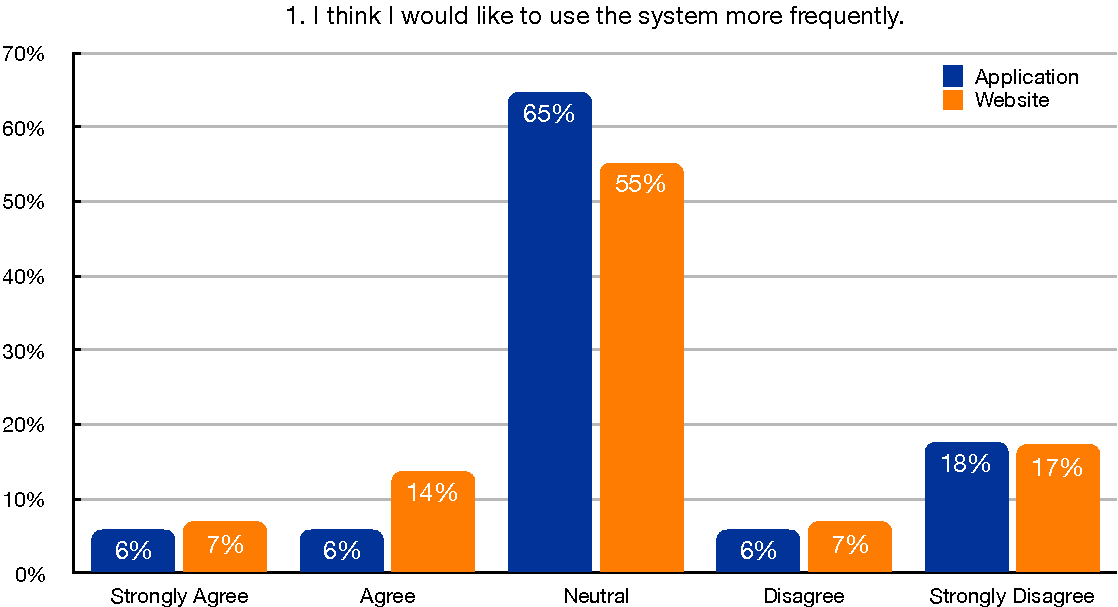
\includegraphics[width=\linewidth]{evaluation/usability-q1.pdf}
  		\caption{Results for question 1.}
  		%\label{fig:plusicon}
	\end{subfigure}\par\bigskip
	
	\begin{subfigure}{.8\textwidth}
  		\centering
  		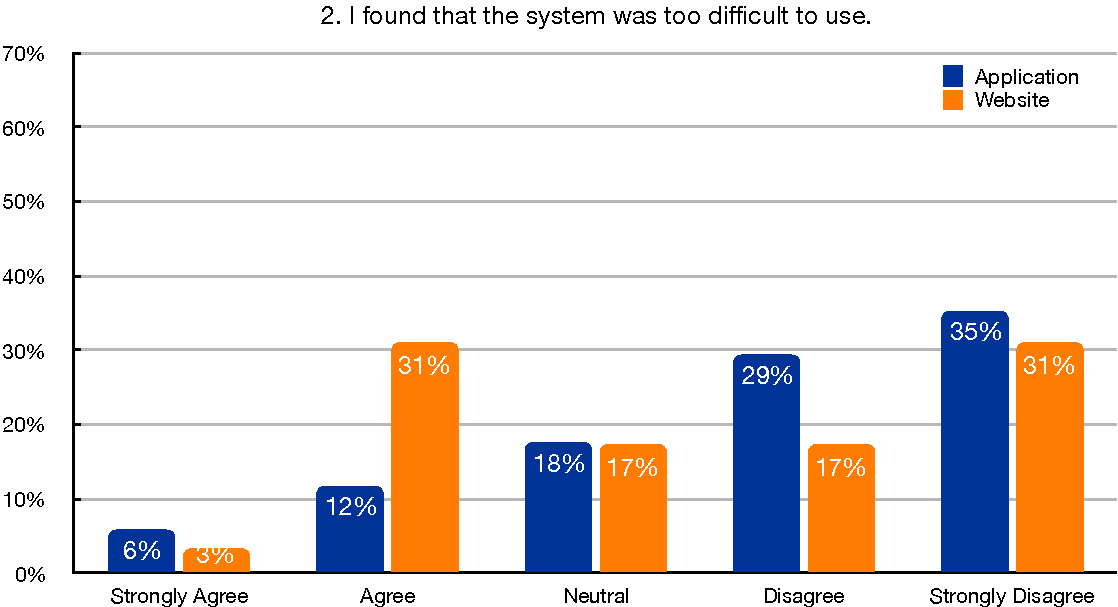
\includegraphics[width=\linewidth]{evaluation/usability-q2.pdf}
  		\caption{Results for question 2.}
  		%\label{fig:editicon}
	\end{subfigure}\par\bigskip
	
	\begin{subfigure}{.8\textwidth}
  		\centering
  		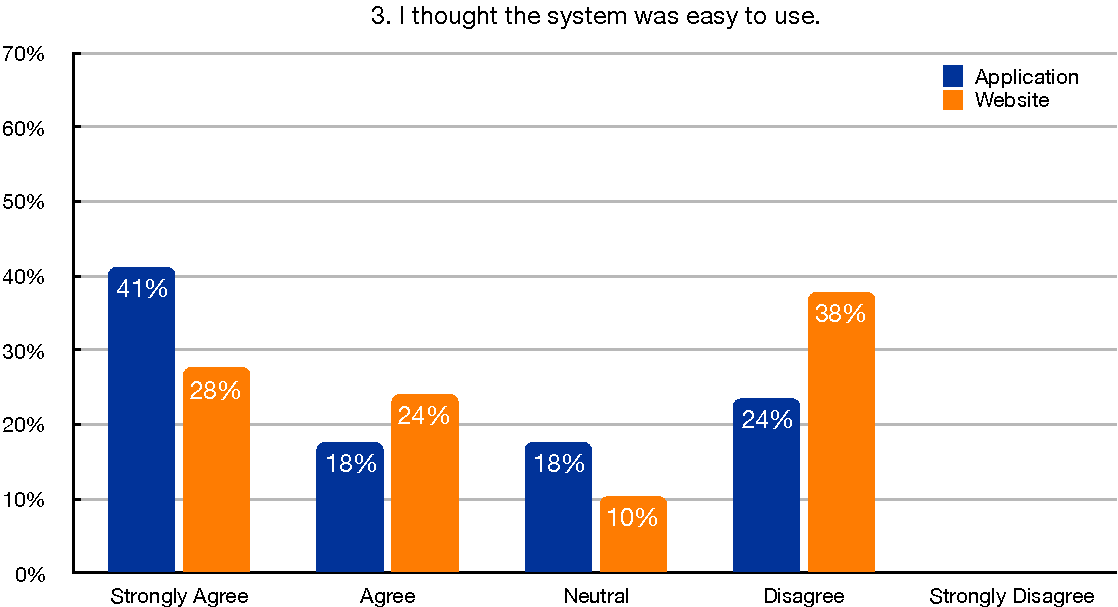
\includegraphics[width=\linewidth]{evaluation/usability-q3.pdf}
  		\caption{Results for question 3.}
  		%\label{fig:plusicon}
	\end{subfigure}
\end{figure}

\begin{figure}[H]\ContinuedFloat
	\centering
	\begin{subfigure}{.8\textwidth}
  		\centering
  		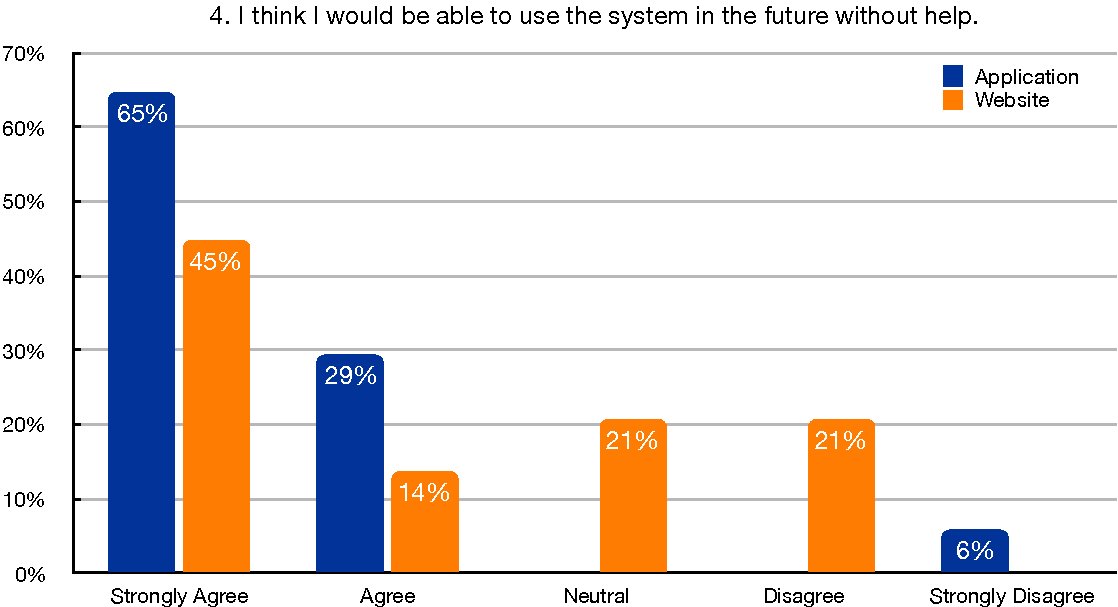
\includegraphics[width=\linewidth]{evaluation/usability-q4.pdf}
  		\caption{Results for question 4.}
  		%\label{fig:editicon}
	\end{subfigure}\par\bigskip
	
	\begin{subfigure}{.8\textwidth}
  		\centering
  		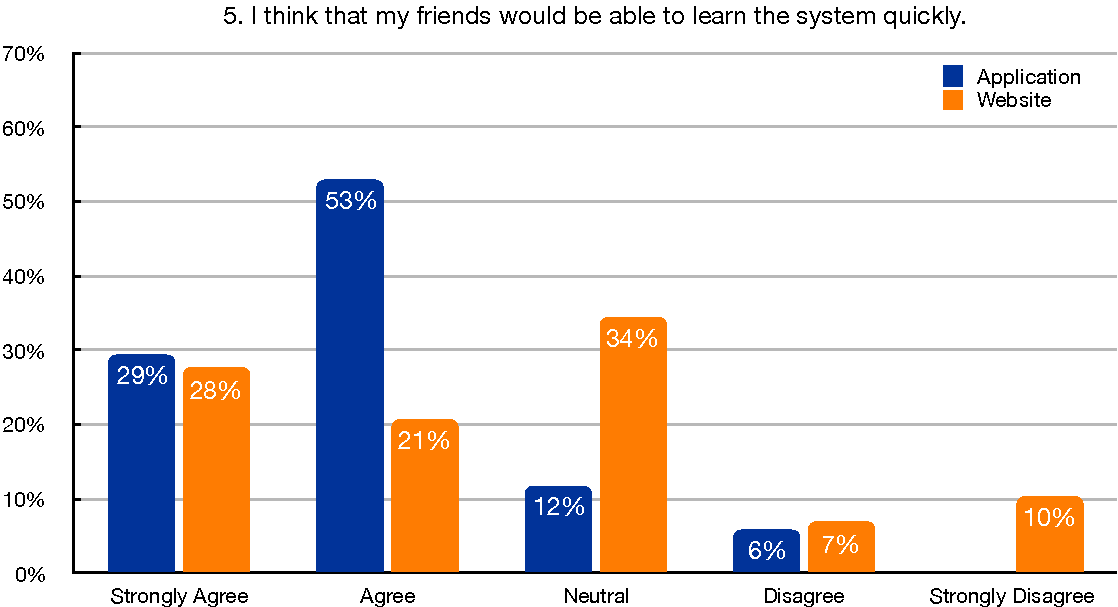
\includegraphics[width=\linewidth]{evaluation/usability-q5.pdf}
  		\caption{Results for question 5.}
  		%\label{fig:plusicon}
	\end{subfigure}\par\bigskip
	
	\begin{subfigure}{.8\textwidth}
  		\centering
  		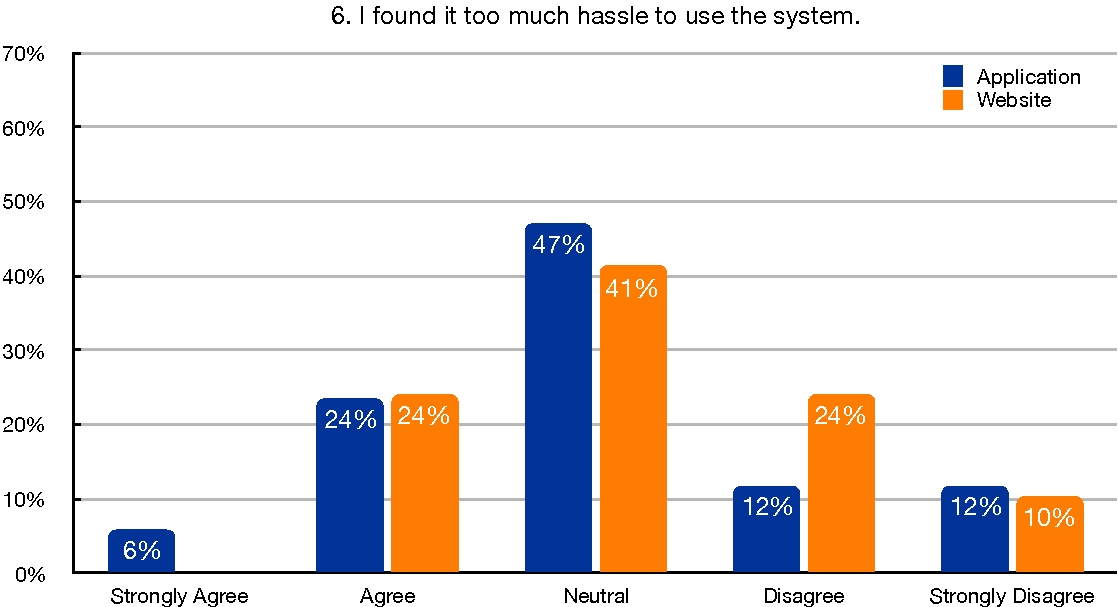
\includegraphics[width=\linewidth]{evaluation/usability-q6.pdf}
  		\caption{Results for question 6.}
  		%\label{fig:editicon}
	\end{subfigure}
\end{figure}

\begin{figure}[H]\ContinuedFloat
	\centering
	\begin{subfigure}{.8\textwidth}
  		\centering
  		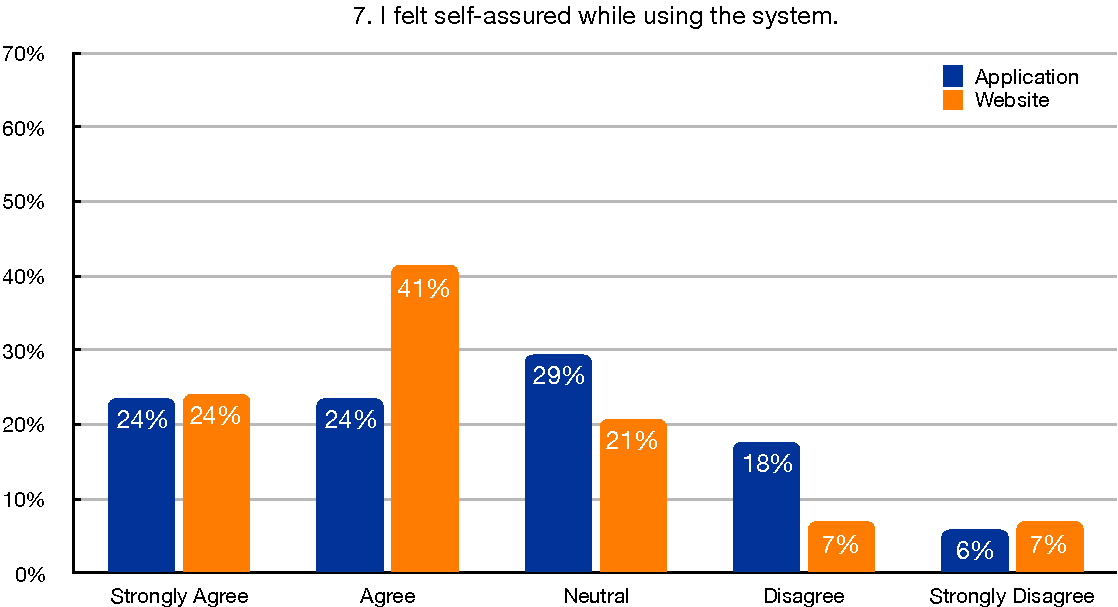
\includegraphics[width=\linewidth]{evaluation/usability-q7.pdf}
  		\caption{Results for question 7.}
  		%\label{fig:plusicon}
	\end{subfigure}\par\bigskip
	
	\begin{subfigure}{.8\textwidth}
  		\centering
  		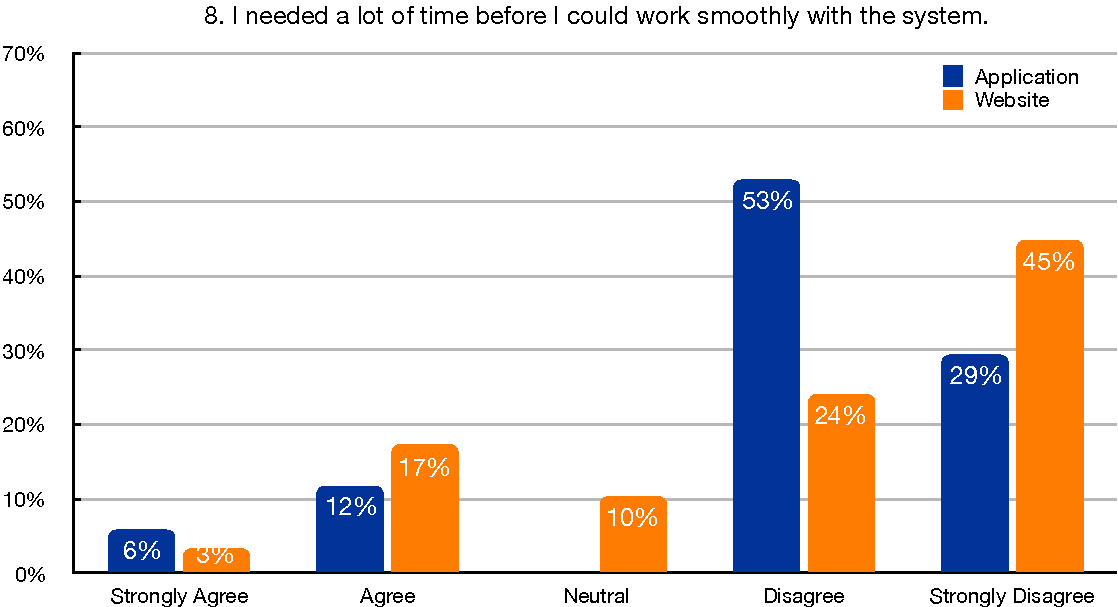
\includegraphics[width=\linewidth]{evaluation/usability-q8.pdf}
  		\caption{Results for question 8.}
  		%\label{fig:editicon}
	\end{subfigure}
	\caption{Usability Results Plateforme DD.}
	\label{fig:evaluation-pdd-usability}
\end{figure}
\clearpage



